%!TEX root =  ..\ekg_7_projektbericht.tex

%Realisierung/Akkumanagement und Versorgungsspannungen

%\setlength{\parindent}{0em} %TODO das habe ich in die Main verschoben um es einheitlich zu halten 

\subsection{Akkumanagement und Versorgungsspannungen}

%TODO Einleitung für das Kapitel, laut Chowanetz soll unter Überschriften immer Text kommen und nicht sofort wieder ne Überschrift
%TODO Abkürzungen ins Abkürzungsverzeichnis schreiben

\subsubsection{Betrachtung der nötigen Energie}

Dieses Unterkapitel behandelt die Analyse der Anforderungen an die Spannungsversorgung eines mobilen EKG Gerätes und erklärt deren Umsetzung.

Im ersten Schritt muss die zu erreichende Laufzeit festgelegt werden. Da das eine Langzeit-EKG Aufnahme möglich sein soll, welche für gewöhnlich 24 Stunden dauert, soll die Versorgung auf 30 Stunden Gerätelaufzeit ausgelegt werden. \\

Um die nötige Kapazität des Akkus festlegen zu können, müssen zunächst sämtliche Hardwarekomponenten mit ihrem durchschnittlichen Verbrauch betrachtet werden. Dies Ergibt sich wie folgt:
\\

\begin{tabular}[h]{l|c|r}
Komponente & Nennspannung & Stromverbrauch während Langzeitaufnahme\\
\hline
Display & 5V & 10mA \\
Bluetooth & 5V & 8mA \\
Cardreader & 5V & 15mA \\
MCU & 3V & 4mA \\
Signalfilterung & 3V & 3mA \\
\end{tabular}
\\
Dadurch ergibt sich eine Leistungsaufnahme von:\\
$ P_{con} = 5V * (10mA + 8mA + 15mA) + 3V * (4mA + 3mA) = 165mW + 21mW = 186mW $

Die Effizienz der noch unbekannten Spannungswandler wird vorläufig mit 80\% angenommen:\\
$P_{draw} = 186mW * \frac{1}{0.8} = 232.5mW $

Multipliziert man den Leistungsbedarf mit der gewünschten Laufzeit so ergibt sich eine nötige Energiemenge von:\\
$W_{Akku} = 232.5mW * 30h = 6975mWh$

\subsubsection{Betrachtung der Zellchemie}

%TODO Quelle für Energiedichte von Zellen suchen

Da Lithium-Ionen Zellen aktuell die höchste Energiedichte für unseren Anwendungsfall liefern, wird diese Art der Zellchemie zu Versorgung des EKG Gerätes verwendet. Um Gefährdungen bei einem Medizinischen Produkt soweit wie möglich vorzubeugen, wird konkret eine Lithium-Polymer-Akku verwendet, welcher Aufgrund der kunststoffähnlichen Eigenschaften des Elektrolyts einen höheren Explosionsschutz sowie bessere Auslaufeigenschaften bietet.
Die Nennspannung dieser Zellen beträgt in der Regel 3,7V. Dadurch ergibt sich eine nötige Ladungsmenge von 
$Q = \frac{6975mWh}{3.7V} = 2051mAh $
Diese Ladungsmenge wird großflächig über die Zellgröße 18560 angeboten, welche Weltweit in Massenfertigung produziert wird und somit keine Finanziellen oder Logistische Probleme darstellt.

%TODO von uns gewählte Zelle beschreiben

\subsubsection{Erzeugung der Unterspannungen}

Eine Li-Po Zelle nimmt während ihrer Entladung Spannungen zwischen 4.2V und 3.2V abhängig vom Ladezustand an. Da sich aus diesem weiten Bereich die Komponenten des EKG-Gerätes nicht zuverlässig versorgen lassen, müssen stabile Zwischenspannungen erzeugt werden. Die erzeugten Spannungen müssen in der Lage sein den maximalen Strom für ihre Baugruppen zu liefern, welcher sich wie folgt zusammensetzt:\\

\begin{tabular}[h]{l|c|r}
Komponente & Nennspannung & Stromverbrauch maximal\\
\hline
Display & 5V & 100mA \\
Bluetooth & 5V & 40mA \\
Cardreader & 5V & 100mA \\
MCU & 3V & 7mA \\
Signalfilterung & 3V & 3mA \\
\end{tabular}
\\
\\
Dies ergibt eine Stromaufnahme von: $I_{3V} = 10mA$ und $I_{5V} = 240mA$
Hierfür bietet sich eine Vielzahl an Möglichkeiten an, welche im Folgendem erläutert werden.\\

Die umfassendste Variante ist die Verwendung eines PMIC (Power Management Integrated Circuit), bei welchem es sich um eine integrierte Schaltung handelt, die alle Anfallenden Aufgaben der Spannungserzeugung übernimmt. Dazu zählen: Battery Management (Überwachung des Ladungszustands der Batterie), Spannungsregulation (Bereitstellen von verschiedenen Unterspannungen), Ladefunktionen. Was auf den ersten Blick als gute Lösung für die gegebenen Anforderungen erscheint, gestaltet sich in der praktischen Umsetzung jedoch schwierig. PMICs kommen idr. im QFN48 Package, welches vergleichsweise groß ist und schwierig zu löten. Somit gestaltet sich das Testen einer Schaltung, welche auf einem PMIC basiert als kompliziert. Hinzu kommen die Vergleichsweise hohen kosten des ICs sowie ein hoher Aufwand an externer Beschaltung. Des weiteren bietet ein PMIC wesentlich mehr Features als für die Projektanforderungen nötig wären, weshalb diese Möglichkeit ausgeschlossen wurde.\\

Als nächste Möglichkeit wurde die Verwendung von Buck- und Boostkonvertern untersucht. Hierbei handelt es sich um integrierte Schaltungen, welche durch zerhacken einer Gleichspannung mittels Transistoren, nutzen der Selbstinduktionseffekte einer Spule sowie anschließende Glättung und Speicherung durch Kondensatoren eine DCDC Wandlung auf höhere oder niedrigere Spannungen ermöglicht. Diese ICs sind verglichen mit PMICs klein, da sie bereits im SOT23 Package erhältlich sind, und können problemlos Ströme im einstelligen Amperebereich bereitstellen. 
Diese Schaltungsart wurde als nächstes mit Bauteilen von Analog Devices in LTSPICE simmuliert. Dabei stellte sich die Erzeugung von 5V durch einen Boost-Konverter als hervorragende Realisierung heraus.

\begin{figure} [!h]
	%\centering
	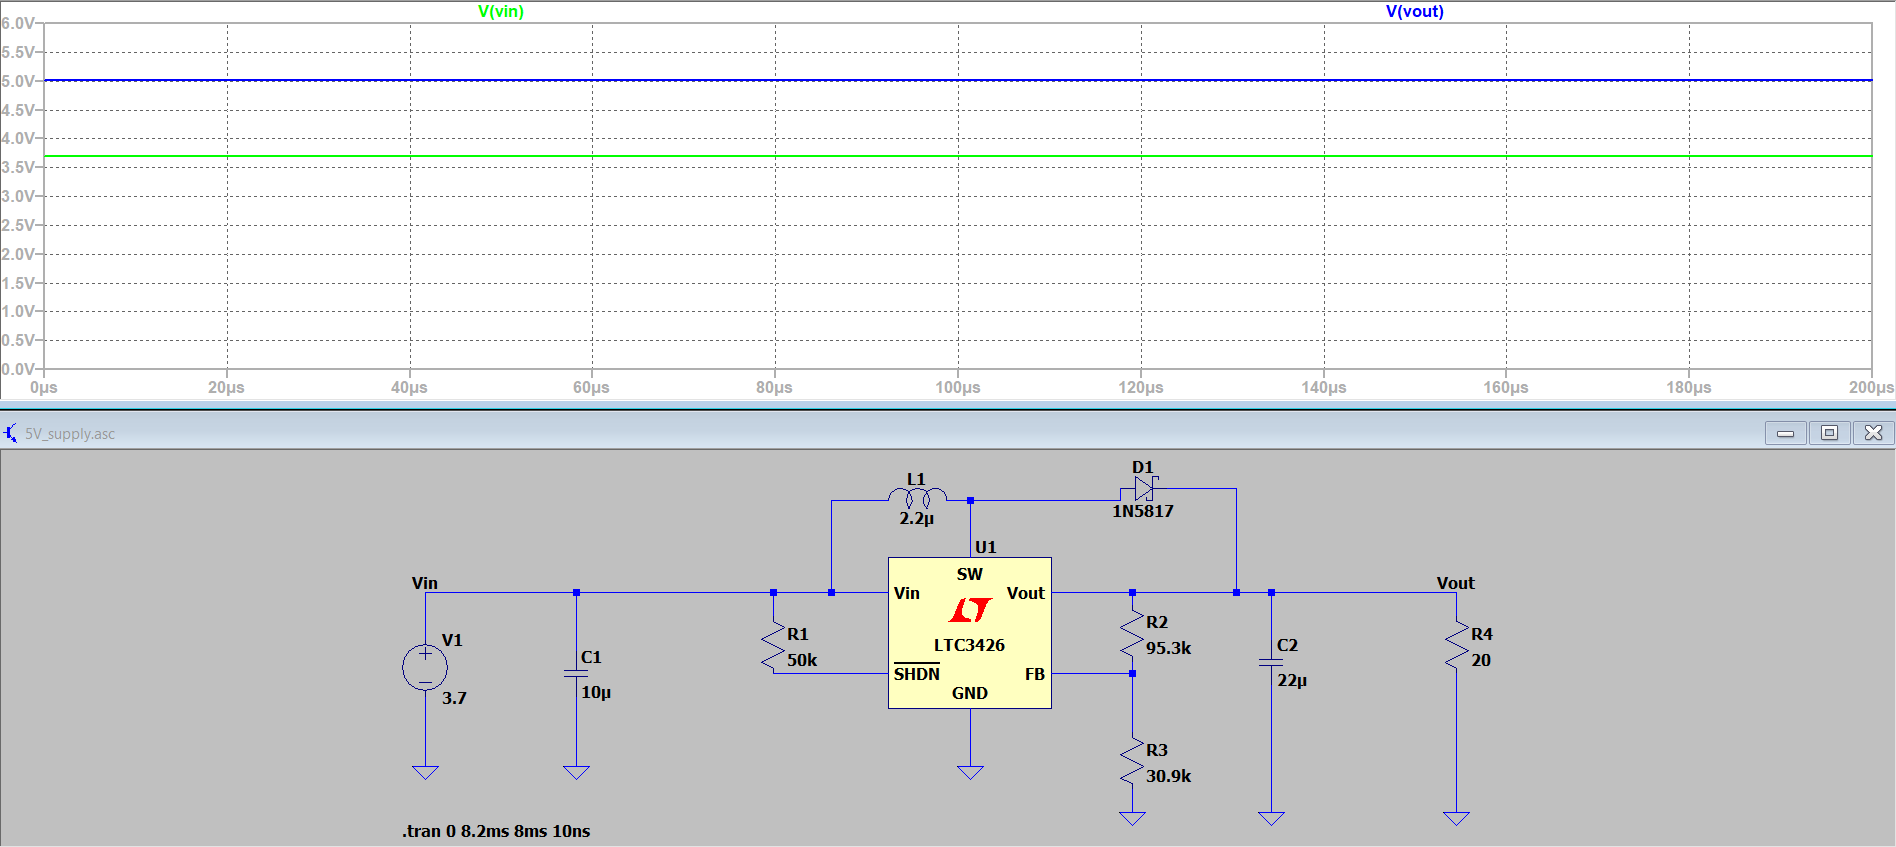
\includegraphics[width=\textwidth] {DCDC_5V_LTSPICE.png}
	\caption{Simulation eines 5V Boost Converters}
	\label{fig_DCDC_5V} 
\end{figure}

Bei der Auswahl eines Boost-Konvertes ist vor allem auf eine hohe Effizienz des ICs sowie einen geringen Eigenverbrauch zu achten. Darüber hinaus gibt es Boost-Konverter mit einem integrierten Enable Pin, welcher nicht nur den IC deaktiviert, sondern auch die Last vollständig vom Eingang abkoppelt. Dies ist überaus nützlich um im Standby Strom zu sparen. Ein Konverter der all diese Anforderungen erfüllt, ist der RP402N501F-TR-FE, welcher bereits ab 0,54€ im Falle einer Massefertigung erhältlich wäre, Ströme bis 800mA sowie eine Effizienz von 90\% - 94\% unterstützt.

Die Erzeugung von 3V durch einen Buck-Konverter ist zwar auch ohne weiteres möglich, allerdings weist diese Schaltungsart bauartbedingt immer eine gewisse Restwelligkeit auf. Da die komplette Analogschaltung zur Aufnahme es EKG Signals mit 3V versorgt wird, sollte hier jede Form von Schwankungen oder Ungenauigkeiten dezimiert werden.
Deshalb fällt die Wahl für die Generierung von 3V auf einen LDO (Low-Dropout-Regler), welcher einen Spannungsabfall über einen internen MOS-FET verursacht und somit die Eingangsspannung auf eine festgelegte Ausgangsspannung herunterregelt. Da in einem LDO keine schaltenden Vorgänge Stattfinden, ist die Restwelligkeit sehr gering. 

\begin{figure} [!h]
	%\centering
	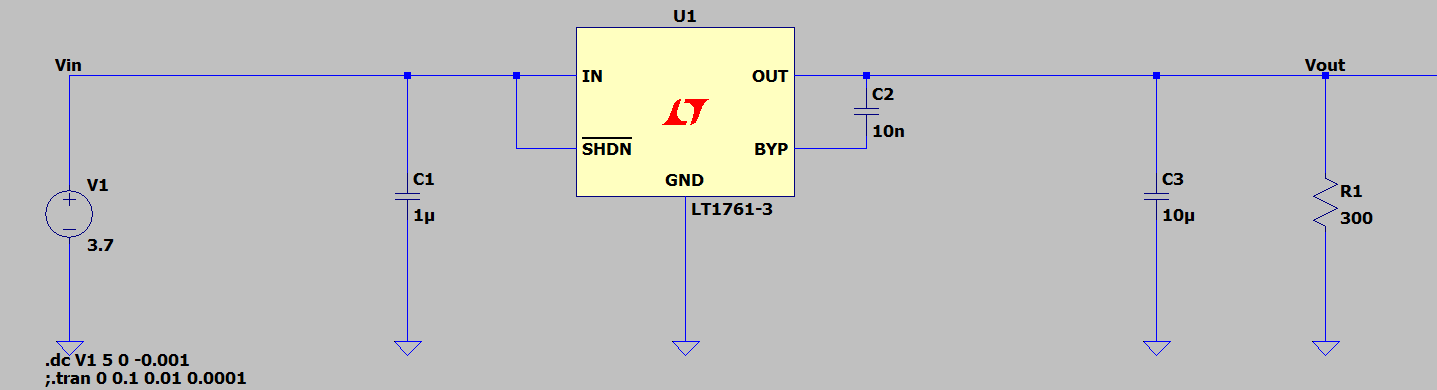
\includegraphics[width=\textwidth] {DCDC_3V_LDO_Shematic.png}
	\caption{Simulationsaufbau 3V LDO}
	\label{fig_DCDC_3V_sch} 
\end{figure}

\begin{figure} [!h]
	%\centering
	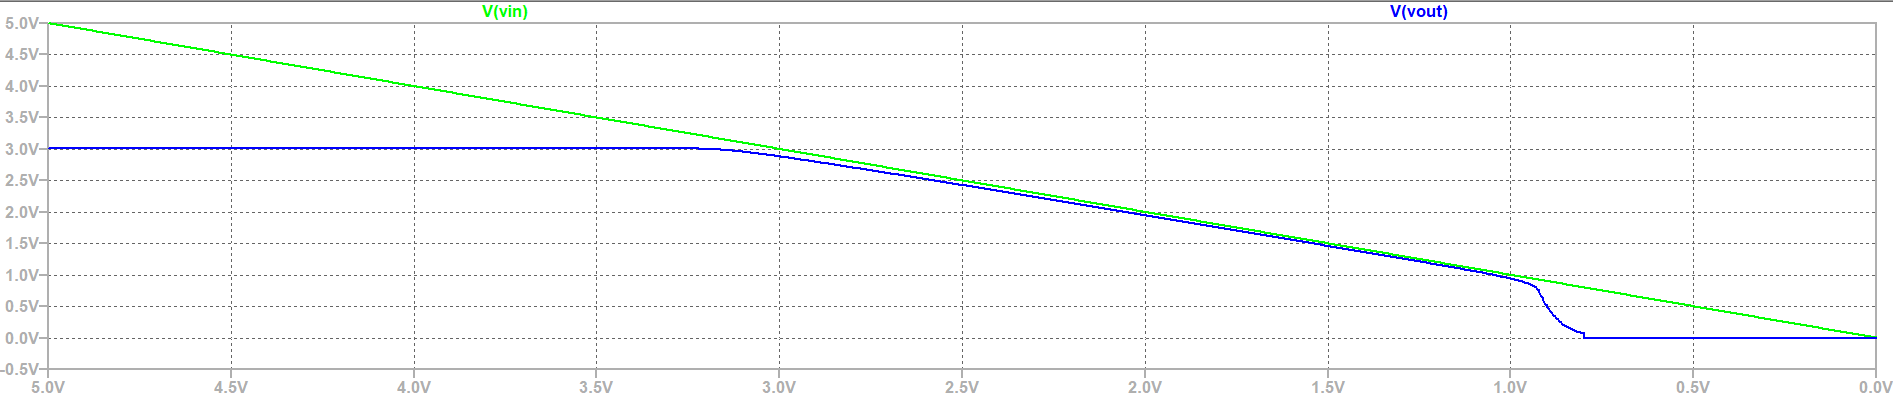
\includegraphics[width=\textwidth] {DCDC_3V_LDO_Plot.png}
	\caption{Ausgang 3V LDO mit fallender Eingangsspannung}
	\label{fig_DCDC_3V_plot} 
\end{figure}


Zu beachten ist jedoch, das ein LDO immer eine minimale Dropout Voltage hat, welche mindestens über ihn abfällt. Somit muss die Eingangsspannung immer größer als die gewünschte Ausgangsspannung plus Dropout Spannung sein. Würde man z.B. eine Ausgangsspannung von 3,3V anstreben und der LDO eine Dropout Voltage von 0,2V besitzen, könnte man den Akku nur bis zu einer Spannung von 3,5V entladen ohne die Ausgangsspannung zu beeinflussen. Deshalb wurde für das EKG-Gerät der LDO TPS79030DBVT mit einer niedrigen Dropout Spannung von 57$\mu$V gewählt. Dieser LDO ist mit einer Restwelligkeit von 56$\mu$V und einem Ruhestrom von 17$\mu$A bestens zur Erfüllung der gestellten Ansprüche geeignet.

\subsubsection{Sicherheitsmaßnahmen}
Die Nutzung von Lithium-Ionen Zellen birgt einige Risiken. Mögliche Gefahren und Maßnahmen zur Reduktion dieser sind:

\begin{enumerate}
	\item Kurzschlüsse: \\
	Als erste Maßnahme hierfür ist der Anschluss der Batterie als Pin Header ausgeführt, wodurch sich am PCB seitigem Ende der Zuleitung eine Buchse befindet. Somit sind die Kontakte im inneren der Buchse geschützt und können nicht durch unachtsame Handhabung Kurzgeschlossen werden. Um bei Kurzschlüssen auf dem Board oder an der Peripherie den Akku zu schützen ist unmittelbar nach dem Header eine Sicherung platziert. Hierfür wurde aus der OMNI-BLOCK Serie von Littelfuse eine 1 Ampere Sicherung mit flinker Auslösecharakteristik gewählt (0154001.DRL). 
	
	\item Verpolung: \\
Um eine Beschädigung der Schaltung durch eine verkehrt eingesetzte Batterie zu verhindern, wodurch Plus- und Minuspol vertauscht wären, ist ein Verpolschutz durch einen PMOS vorhanden. Der Drain-Anschluss liegt hierbei an der Batterie währen der Source-Anschluss dem Rest der Schaltung zugewandt ist. Dadurch ist Bei korrekter Polung der Body-Diode von Drain nach Source leitend. Das Gate ist über einen Widerstand mit dem Ground verbunden, wodurch im Normalbetrieb eine negative Gate-Source Spannung anliegt und den Transistor komplett durchsteuert. Im Fall einer Verpolung ist die Body-Diode nicht leitend und es entsteht keine Potentialdifferenz zwischen Gate und Source. Der FET sperrt und die Schaltung ist geschützt.

	\item Überspannung:\\
	Überspannungen z.B. durch eine elektrostatische Entladung (ESD) beim wechseln der Batterie können der Schaltung Schaden zufügen. Zur Prävention ist am Spannungeingang eine Bidirektionale Transient Voltage Suppressor (TVS) Diode verbaut, welche Spannungen über 9V schnell nach Ground ableitet.
	
	\item Tiefenentladung:\\
	Eine Entladung auf Spannungen außerhalb der Spezifikation des Akkus können zu dessen Zerstörung führen. Aus diesem Grund wird fortwährend die aktuelle Akkuspannung des Geräts durch die MCU gemessen und ein Einschalten des Geräts wird nur bei ausreichender Spannung erlaubt. Zusätzlich wird ein Akku mit integrierter Schutzbeschaltung verwendet, welche ebenso einen Tiefentladungsschutz enthält.

\end{enumerate}

